\documentclass{article}

\usepackage[preprint]{neurips_2024}

\usepackage[utf8]{inputenc} % allow utf-8 input
\usepackage[T1]{fontenc}    % use 8-bit T1 fonts
\usepackage{hyperref}       % hyperlinks
\usepackage{url}            % simple URL typesetting
\usepackage{booktabs}       % professional-quality tables
\usepackage{amsfonts}       % blackboard math symbols
\usepackage{nicefrac}       % compact symbols for 1/2, etc.
\usepackage{microtype}      % microtypography
\usepackage{xcolor}         % colors
\usepackage{graphicx}       % include graphics
\usepackage{subcaption}     % subfigures
\usepackage{amsmath}        % math symbols
\usepackage{amssymb}        % additional math symbols
\usepackage{algorithm}
\usepackage{algorithmic}



\title{Topology-Guided Protein Design}

\author{
  Anna Su\thanks{GitHub repository for the project can be found at \url{https://github.com/annasu1225/knotprot_design}. YouTube presentation: \url{https://youtu.be/P7KVEJcRkBE}.} \\
  Department of Computer Science\\
  Yale University\\
  New Haven, CT 06520 \\
}

\begin{document}

\maketitle

\section{Abstract}

Knotted proteins exhibit rare and highly conserved topological structures that are associated with enhanced mechanical and thermal stability, slow unfolding kinetics, and resistance to degradation.
Despite growing interest in exploiting protein topology for design, existing generative frameworks lack mechanisms to directly control non-differentiable topological properties.
In this work, we present a computational framework for topology-guided protein design that integrates knot-theoretic constraints into the ESM3 multimodal protein language model using derivative-free guidance.
We demonstrate that a non-differentiable knot invariant—the Alexander polynomial—can be incorporated as a reward signal during generative decoding, enabling the de novo design of a trefoil-knotted protein and the mutant design of an unknotted variant.
Our results establish a proof-of-concept for using discrete topological invariants to guide large protein generative models without retraining or differentiable surrogates, opening new directions for geometry- and topology-aware protein design.

\section{Introduction}

Property-guided protein design has emerged as a central challenge in computational biology, driven by the need to generate sequences that simultaneously satisfy functional, structural, and physical constraints \cite{Tagasovska2022,Hong2024,Luo2025}.
Recent advances in generative models, particularly diffusion and language-model-based approaches, have enabled unprecedented exploration of protein sequence and structure space \cite{Hayes2025}.
However, most existing methods rely on differentiable proxy objectives or model fine-tuning, limiting their applicability to properties that admit smooth approximations.

Protein geometry and topology provide a complementary and underexplored axis for design.
Proteins with specific geometric or topological features have been shown to exhibit distinct stability, folding, and functional characteristics \cite{Sukowska2008,Hsu2024,Madsen2025}.
In particular, knotted proteins—whose backbones form nontrivial mathematical knot types—are associated with increased mechanical stability and resistance to thermal unfolding \cite{Sukowska2012,Faisca2015,Lim2015}.
Despite their potential advantages, deeply knotted proteins remain rare in nature and difficult to design experimentally \cite{King2010,Doyle2023}.

From a machine learning perspective, knot type represents a fundamentally topological property: it is invariant under continuous deformations and cannot be captured by local geometric descriptors alone.
Moreover, commonly used knot invariants, such as the Alexander polynomial \cite{Alexander1928}, are discrete and non-differentiable with respect to atomic coordinates.
This makes them incompatible with standard gradient-based conditional generation techniques.

In this project, we introduce a topology-guided protein design framework that integrates knot-theoretic rewards into ESM3 using derivative-free guidance \cite{Li2024}.
By computing the Alexander polynomial from generated protein backbones using the Topoly package \cite{Dabrowski-Tumanski2021}, we successfully guide ESM3 to generate a de novo trefoil-knotted protein.
Our contributions are threefold:
(1) we demonstrate that non-differentiable topological invariants can be used as effective guidance signals;
(2) we show that derivative-free decoding enables topology-aware control of large protein language models without retraining; and
(3) we provide a concrete example of trefoil knot design driven purely by mathematical knot constraints.

\section{Background and Related Work}

\paragraph{Knots in proteins.}
A protein backbone can be viewed as a piecewise-smooth spatial curve embedded in $\mathbb{R}^3$.
By closing the open chain using standard closure procedures, one can assign a knot type to the protein conformation \cite{Faisca2015}.
Although most proteins are unknotted, a small but significant subset exhibit trefoil ($3_1$), figure-eight ($4_1$), or more complex knot types, often conserved across families \cite{Sukowska2012,Dabrowski-Tumanski2019}.

\paragraph{Knot invariants and the Alexander polynomial.}
Knot invariants are quantities that remain unchanged under ambient isotopy, meaning they stay the same even when a knot is continuously stretched, twisted, or deformed 
in space without cutting or self-intersection, serving as powerful tools to tell different knots apart \cite{Adams2004}. See Appendix \ref{app:alexander} for a demonstration of computation. 
Among the earliest and most widely used is the Alexander polynomial $\Delta_K(t)$ \cite{Alexander1928}, which assigns a Laurent polynomial to a knot $K$.
While not complete, the Alexander polynomial is sufficient to distinguish trefoil knots from the unknot and many other simple knot types.
Importantly, because it is a topological invariant and its value changes only when the knot's topology changes, for example, via a Reidemeister move, the function mapping a geometric configuration to its polynomial value is a step function, not a smooth or continuous one, 
meaning that it is discrete and non-differentiable with respect to geometric perturbations, making it unsuitable for gradient-based optimization but ideal for derivative-free guidance.

\paragraph{Property-guided protein generation.}
Prior work in conditional protein design has focused primarily on differentiable objectives or learned surrogate models, including energy-based models \cite{Tagasovska2022}, multi-objective evolutionary optimization \cite{Hong2024}, and Pareto-optimal sampling strategies \cite{Luo2025}.
These approaches excel at balancing multiple biochemical properties but typically operate in sequence space and do not explicitly control global topological structure.

\paragraph{Knotted protein design.}
Experimental and computational efforts have demonstrated the feasibility of designing knotted proteins by carefully engineering folding pathways \cite{King2010,Doyle2023}.
However, these methods rely on handcrafted backbone construction and extensive biophysical validation.
To our knowledge, no prior work has demonstrated generative, topology-guided protein design using large pretrained models and explicit knot invariants.


\section{Methods and Models}

\paragraph{ESM3 generative model.}
ESM3 is a multimodal protein language model trained jointly on sequence, structure, and functional annotations \cite{Hayes2025}.
It supports iterative structure generation by sampling backbone coordinates conditioned on partial context.
Notably, ESM3 can be used as a frozen generative prior, making it suitable for post-hoc guidance methods.

\paragraph{Derivative-free guidance.}
We adopt the derivative-free guidance framework proposed by Li et al.\ \cite{Li2024}, which modifies the decoding process of diffusion or autoregressive models using a soft value function.
At each generation step, multiple candidate continuations are sampled, evaluated using a reward function, and reweighted to bias future sampling toward high-reward trajectories.
This approach avoids both model fine-tuning and differentiable surrogate construction.

\paragraph{Topological reward function.}
For each generated protein backbone, we compute a closed-chain representation and evaluate its Alexander polynomial using Topoly \cite{Dabrowski-Tumanski2021}.
The reward function assigns higher scores to structures whose polynomial matches that of the target knot type and penalizes unknotted or ambiguous configurations.
Because the Alexander polynomial is non-differentiable and discrete, derivative-free guidance is essential.

\paragraph{Guided decoding procedure.}
Starting from an unconditioned ESM3 generation, we iteratively apply derivative-free guidance during structure sampling.
At each step, candidate structures are evaluated for knot type, and the sampling distribution is adjusted to increase the likelihood of trefoil-consistent trajectories.
No gradients are computed with respect to ESM3 parameters or atomic coordinates.


\section{Empirical and Theoretical Results}

\paragraph{De novo trefoil protein generation.}
Using derivative-free topology-guided decoding, we successfully generated a protein backbone whose Alexander polynomial matches that of a trefoil knot ($3_1$).
The backbone was generated entirely \emph{de novo} using ESM3, with the knot type label ``$3_1$'' provided as a conditioning signal during guided decoding and the sequence length restricted to 256 residues.
No wildtype sequence, structural template, or fold constraint was supplied at any stage of generation.

This result is notable given the extreme rarity of knotted proteins in natural datasets.
Proteins exhibiting nontrivial knot types constitute approximately 1\% of structures deposited in the Protein Data Bank, with the majority forming simple trefoil knots and only a handful exhibiting higher-order knotting.
As a consequence, ESM3—despite its large-scale pretraining—should not be expected to have learned explicit representations of knotted protein topologies.
The successful generation of a trefoil knot therefore indicates that the model can be steered into rare and topologically complex regions of structure space when equipped with an appropriate non-differentiable reward signal.

To validate the knot type of the generated backbone, we performed explicit topological analysis using KnotPlot.
Because protein backbones are open chains, we manually closed the N- and C-termini using a standard closure procedure designed to avoid introducing artificial crossings.
Specifically, the termini were extended and connected in a manner that preserves the ambient isotopy class of the backbone.
Following closure, the resulting loop was subjected to dynamical relaxation in KnotPlot, allowing the chain to simplify under tension while preserving topology.
This relaxation process reveals a stable trefoil knot core embedded within the backbone, consistent with known trefoil protein geometries.
A video of the full dynamical relaxation procedure is provided in the accompanying GitHub repository.

Figure~\ref{fig:trefoil_protein} illustrates the generated backbone, the manual closure procedure, and the simplified trefoil knot obtained after topological reduction.
Together, these results provide strong evidence that derivative-free guidance enables ESM3 to generate genuinely knotted protein structures, rather than superficial or closure-induced artefacts.

\begin{figure}[h!]
    \centering
    \begin{subfigure}[t]{0.32\textwidth}
        \centering
        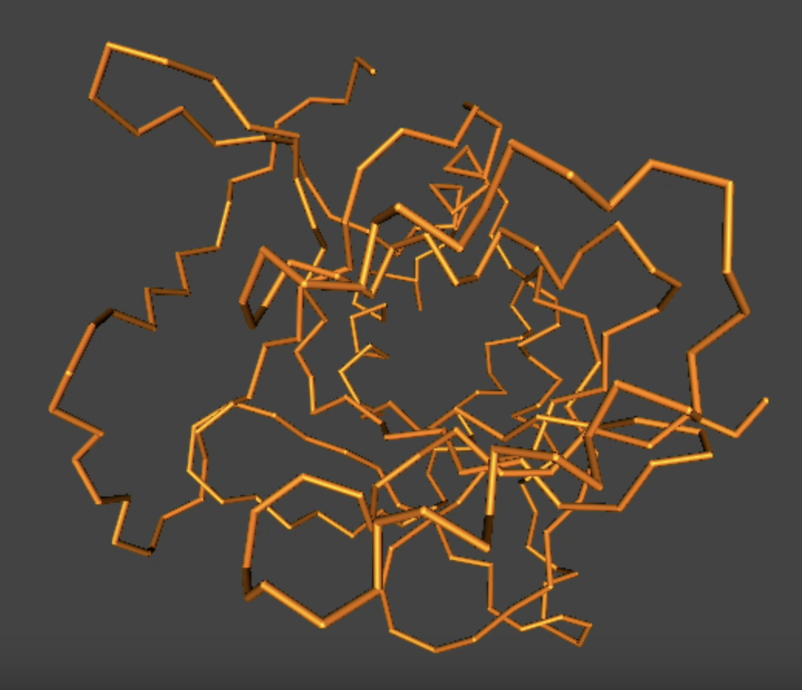
\includegraphics[height=3.2cm]{Figures/backbone_structure.png}
        \caption{}
    \end{subfigure}
    \hfill
    \begin{subfigure}[t]{0.32\textwidth}
        \centering
        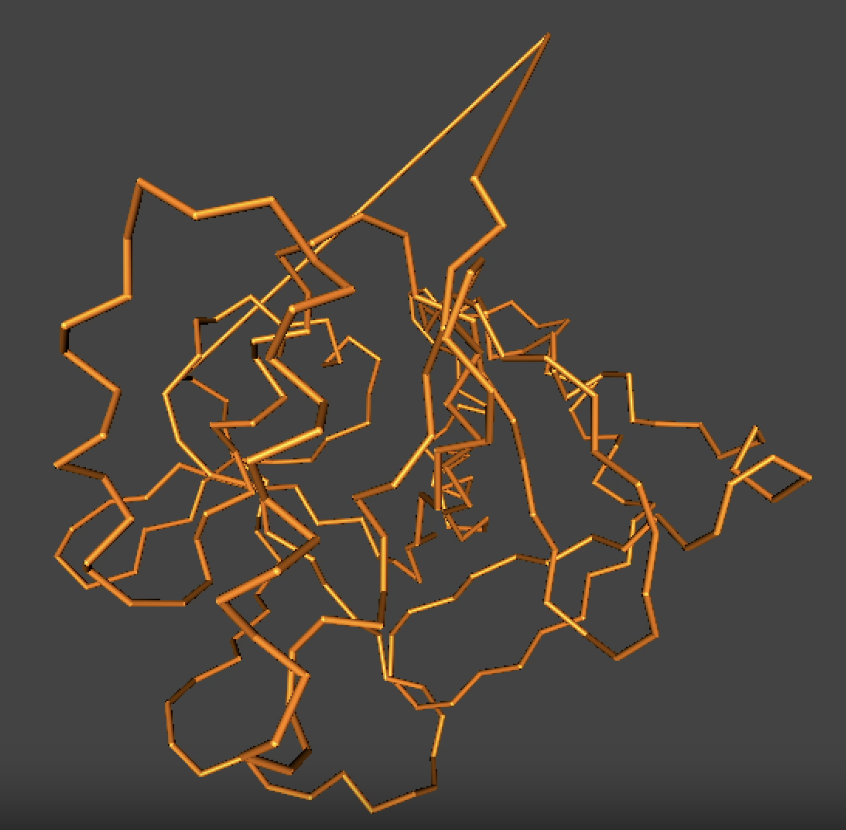
\includegraphics[height=3.2cm]{Figures/manual_closure.png}
        \caption{}
    \end{subfigure}
    \hfill
    \begin{subfigure}[t]{0.32\textwidth}
        \centering
        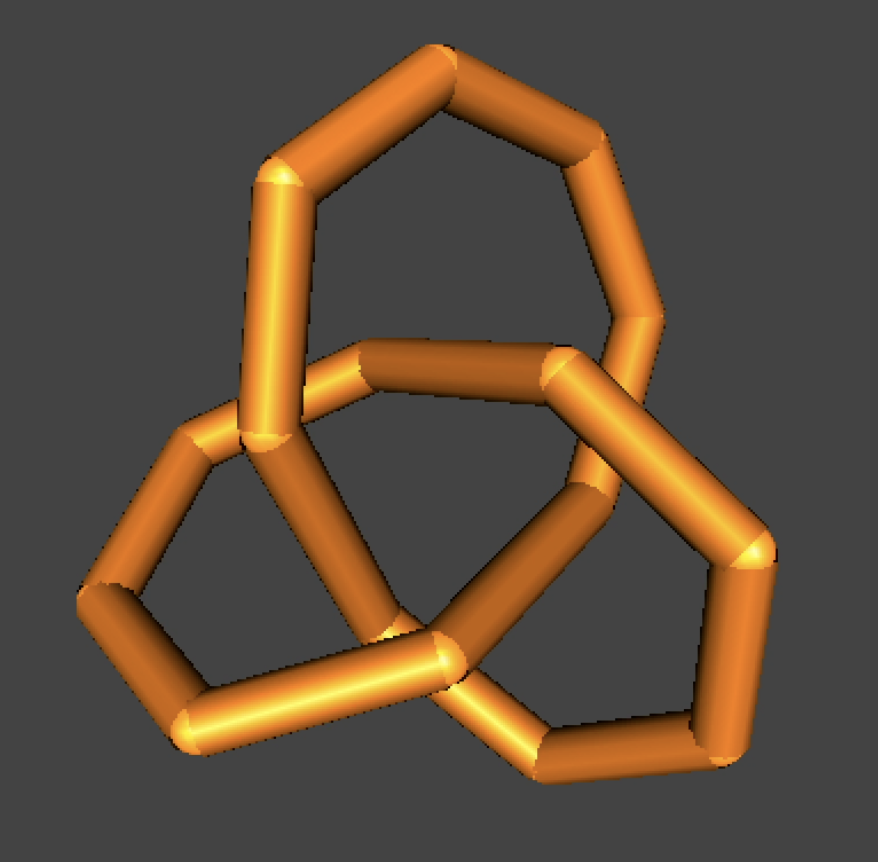
\includegraphics[height=3.2cm]{Figures/trefoil_knot.png}
        \caption{}
    \end{subfigure}

    \caption{
    (a) Generated protein backbone structure.
    (b) Manual closure of the protein ends for knot analysis.
    (c) Simplified trefoil knot representation after applying dynamical relaxation in KnotPlot.
    }
    \label{fig:trefoil_protein}
\end{figure}

\paragraph{Unknotting a trefoil protein.}
While designing knotted proteins can enhance stability, the inverse problem—designing unknotted mutants of naturally knotted proteins —is equally important from biological and clinical perspectives.
Controlled unknotting enables systematic investigation of how knot topology influences protein folding pathways, kinetic trapping, thermodynamic stability, and biological function.
Because knots introduce long-range topological constraints and complex folding landscapes, they can slow folding, increase misfolding risk, and create metastable intermediates, all of which are implicated in disease and evolutionary selection.
The ability to selectively remove knotting while preserving overall fold therefore offers a powerful tool for studying protein evolution, engineering faster-folding variants, and designing therapeutics that mitigate misfolding-related pathologies.

To demonstrate this capability, we performed conditional design of an unknotted mutant starting from a naturally trefoil-knotted protein.
The wildtype sequence was provided as context, and the topology label ``$0_1$'' was supplied as the conditioning signal during derivative-free guided decoding.
No explicit structural constraints enforcing unknotting were imposed beyond the topological reward.

The resulting design was predicted to adopt a stable, unknotted structure as assessed using ESMFold (Figure~\ref{fig:unknotted_design}).
Structural analysis confirmed the absence of nontrivial entanglement, while maintaining a compact and well-ordered backbone.
The predicted model achieved a mean pLDDT score of 0.74 and a pTM score of 0.74, indicating satisfactory local confidence and global structural consistency.
These results suggest that topology-guided decoding can not only induce rare knotted structures, but also selectively remove topological constraints from existing proteins, enabling controlled exploration of how knotting modulates protein behavior.

\begin{figure}[h!]
    \centering
    \centering
    \begin{subfigure}[t]{0.44\textwidth}
        \centering
        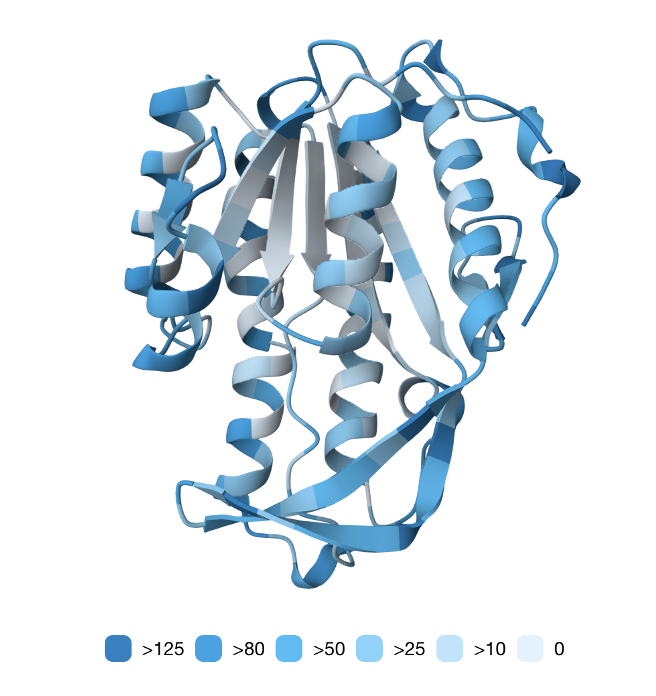
\includegraphics[height=5.2cm]{Figures/unknot_mutant_SASA.png}
        \caption{}
    \end{subfigure}
    \hfill
    \begin{subfigure}[t]{0.44\textwidth}
        \centering
        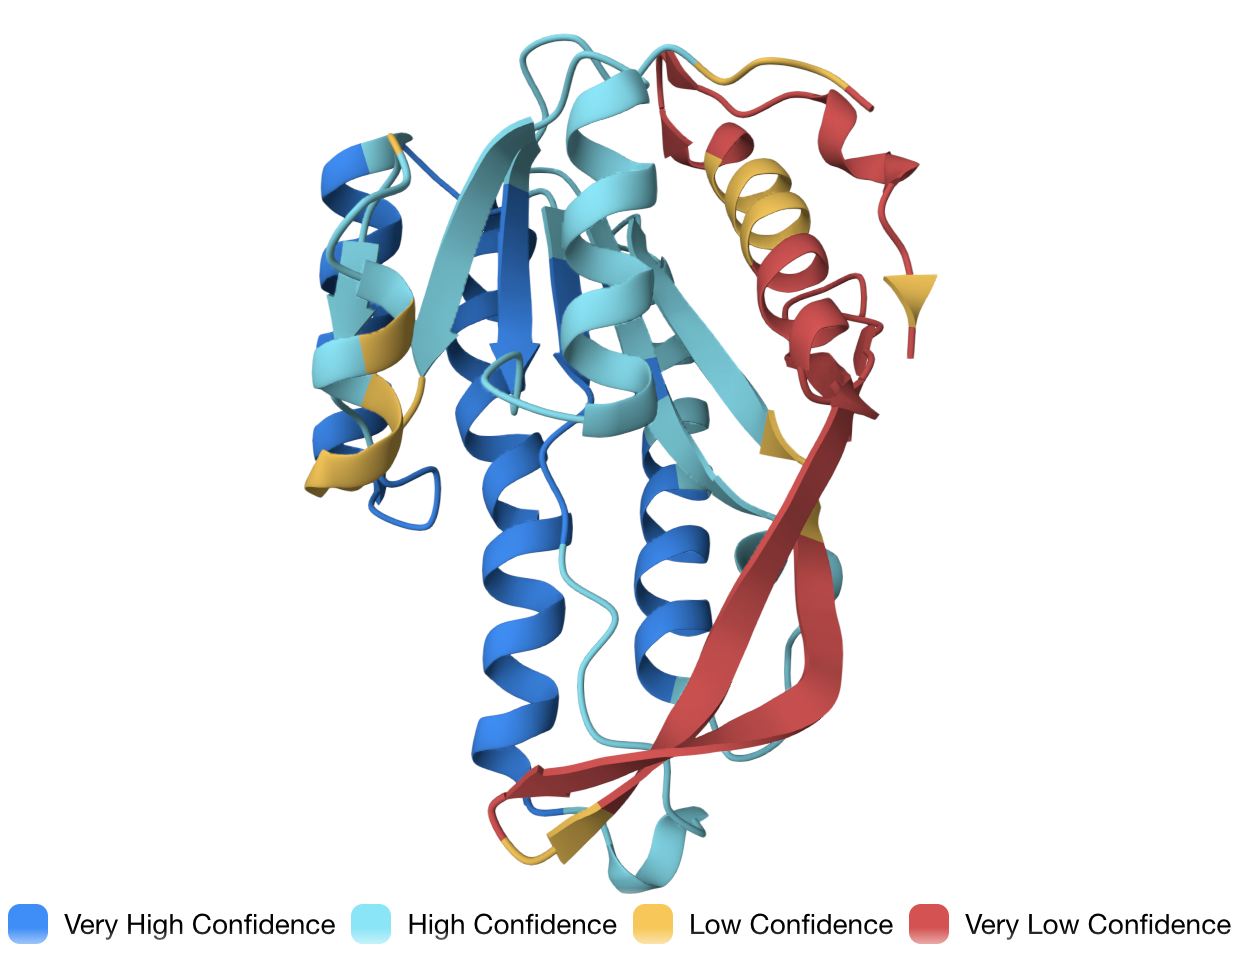
\includegraphics[height=5.2cm]{Figures/unknot_mutant_plddt.png}
        \caption{}
    \end{subfigure}
    \caption{ESMFold predicted structure of the unknotted mutant designed from a trefoil-knotted wildtype protein colored by (a) SASA value and (b) pLDDT score.}
    \label{fig:unknotted_design}
\end{figure}


\section{Conclusion and Future Work}

We introduced a topology-guided protein design framework that integrates knot-theoretic invariants into ESM3 using derivative-free guidance.
By leveraging the Alexander polynomial as a non-differentiable reward, we successfully generated a de novo trefoil-knotted protein and an unknotted mutant.
This work highlights the feasibility of incorporating discrete, global topological constraints into large protein generative models.

Several limitations remain. The current framework does not incorporate binding affinity, pocket curvature, or 
kinetic accessibility which are all properties related to protein topology. We are currently exploring conditioning protein design on binding pocket gaussian curvature and linking-number profiles.
Future work could incorporate these properties to develop ensemble-based topological and geometrical measures. 

An important alternative direction is conditional generation using flow matching or diffusion models trained on protein properties.
Such models could learn smooth latent representations of knot classes and geometric profiles, potentially improving sampling efficiency and robustness.
However, this would require curated datasets of knotted proteins and substantial retraining.
In contrast, derivative-free guidance offers immediate flexibility and compatibility with existing pretrained models.
This work suggests that topology-aware machine learning may play a critical role in future protein design, enabling control over properties that lie beyond local geometry.

\bibliographystyle{unsrt}
\bibliography{references}

\appendix

\setcounter{figure}{0}
\renewcommand{\thefigure}{S\arabic{figure}}

\section{Alexander Polynomial: Trefoil Example}
\label{app:alexander}

We briefly demonstrate the computation of the Alexander polynomial for the trefoil knot ($3_1$), 
illustrating its use as a discrete topological invariant.

\begin{figure}[h!]
    \centering
    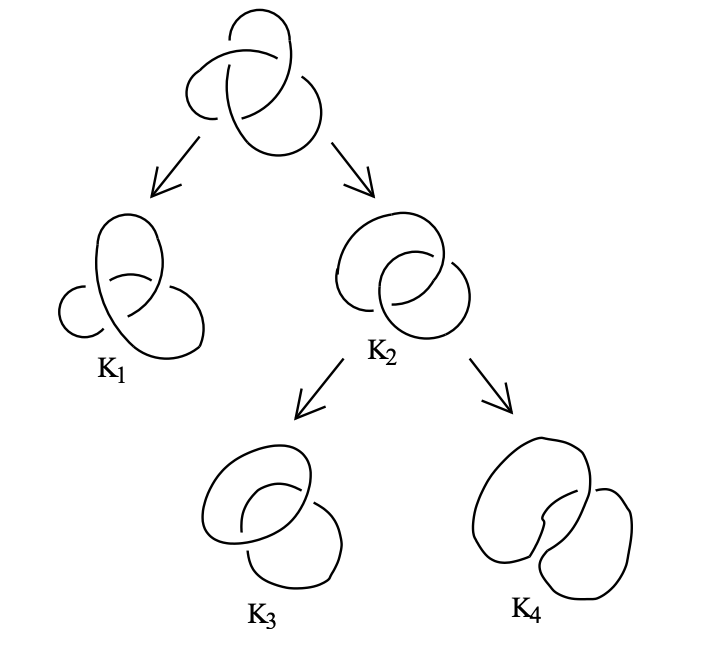
\includegraphics[width=0.4\textwidth]{Figures/ap.png}
    \caption{Trefoil knot and its skein relation components.}
    \label{fig:trefoil_ap}
\end{figure}

\paragraph{Skein relation.}
The Alexander polynomial $\Delta_K(t)$ is defined (up to $\pm t^k$) by
\begin{align}
\Delta_{\text{unknot}}(t) &= 1, \\
\Delta_{L_+}(t) - \Delta_{L_-}(t)
+ \left(t^{1/2} - t^{-1/2}\right)\Delta_{L_0}(t) &= 0,
\end{align}
where $L_+$, $L_-$, and $L_0$ differ locally at a single crossing.

\paragraph{Trefoil reduction.}
Applying the skein relation to a trefoil crossing yields
\begin{equation}
\Delta_{3_1}(t)
= \Delta_{K_1}(t)
- \left(t^{1/2} - t^{-1/2}\right)\Delta_{K_2}(t),
\end{equation}
where $K_1$ is isotopic to the unknot and $\Delta_{K_1}(t)=1$.
Reducing $K_2$ again gives
\begin{equation}
\Delta_{K_2}(t)
= \Delta_{K_3}(t)
+ \left(t^{1/2} - t^{-1/2}\right)\Delta_{K_4}(t),
\end{equation}
with $\Delta_{K_3}(t)=0$ (two-component unlink) and $\Delta_{K_4}(t)=1$.

\paragraph{Result.}
Substituting yields
\begin{align}
\Delta_{3_1}(t)
&= 1 - \left(t^{1/2} - t^{-1/2}\right)^2 \\
&= t^{-1} - 1 + t.
\end{align}

This polynomial uniquely identifies the trefoil knot among simple knot types and serves as the non-differentiable topological reward used in our guided protein generation.

\section{Derivative-Free Guidance for ESM3}
\label{app:dfg_esm3}

We summarize the soft value-based decoding (SVDD) framework of \cite{Li2024} and its application to ESM3 generation.
SVDD enables optimization of non-differentiable rewards while preserving the pretrained model prior.

\subsection{Reward-tilted target distribution}
Let $p_\theta(x_0\mid c)$ denote the pre-trained prior, the original ESM3's distribution over final outputs $x_0$ conditioned on context $c$ (e.g. desired fold or topology).
Given a non-differentiable reward $r(x_0)$, SVDD targets
\begin{equation}
p^\star(x_0\mid c) \propto p_\theta(x_0\mid c)\exp\!\big(\beta r(x_0)\big),
\label{eq:svdd_target}
\end{equation}
where $\beta$ controls guidance strength.

\subsection{Soft value function}
ESM3 generation proceeds through intermediate states $x_T,\dots,x_0$ with transitions
\begin{equation}
\pi_\theta(x_{t-1}\mid x_t,c).
\end{equation}
Define the soft value function
\begin{equation}
V_t(x_t,c)
=
\mathbb{E}\!\left[\exp\!\big(\beta r(x_0)\big)\mid x_t,c\right],
\label{eq:svdd_value}
\end{equation}
where the expectation is over model rollouts to completion.
The optimal value-weighted transition is
\begin{equation}
\pi^\star(x_{t-1}\mid x_t,c)
\propto
\pi_\theta(x_{t-1}\mid x_t,c)\,V_{t-1}(x_{t-1},c).
\label{eq:svdd_policy}
\end{equation}

\subsection{Iterative decoding}
SVDD approximates sampling from \eqref{eq:svdd_policy} via per-step importance sampling.

\begin{algorithm}[h]
\caption{SVDD-style derivative-free decoding}
\label{alg:svdd}
\begin{algorithmic}[1]
\STATE Initialize $x_T$
\FOR{$t=T,\dots,1$}
    \STATE Sample $\{x_{t-1}^{(m)}\}_{m=1}^M \sim \pi_\theta(\cdot\mid x_t,c)$
    \STATE Compute $w^{(m)} \propto \widehat V_{t-1}(x_{t-1}^{(m)},c)$
    \STATE Select $x_{t-1}$ by categorical sampling over $\{w^{(m)}\}$
\ENDFOR
\STATE \textbf{return} $x_0$
\end{algorithmic}
\end{algorithm}

\subsection{Value estimation}
For non-differentiable rewards, $V_t$ is estimated using short Monte Carlo rollouts:
\begin{equation}
\widehat V_t(x_t,c)
=
\frac{1}{K}\sum_{k=1}^K
\exp\!\big(\beta r(x_0^{(k)})\big),
\qquad
x_0^{(k)}\sim\pi_\theta(\cdot\mid x_t,c).
\end{equation}

\subsection{Application to ESM3}
Although originally derived for diffusion models, SVDD only requires an iterative generative process and reward evaluation.
ESM3 supports iterative refinement of sequence and structure, inducing $\pi_\theta(x_{t-1}\mid x_t,c)$ and enabling SVDD without retraining.
In our work, $r(x_0)$ is a discrete knot invariant (Alexander polynomial), making derivative-free guidance essential.

\end{document}